\section{무곱셈 희소 스파이크 구동 커널}\label{sec:kernel}

\subsection{항등식과 비트 동일성}\label{sec:identity}

이 파이프라인의 모든 합성곱 입력은 이진이다: CPL1 입력은 인코더
출력 $\{0, 32{,}767\}$, CPL2 입력은 LIF1 스파이크 $\{0, S_1\}$이며,
제로 패딩은 비발화와 동일하다. 입력이 $\{0, S\}$이면 내적이
붕괴한다:
\begin{equation}
\sum_{k=0}^{r-1} w_k\, x_k \;=\; S \cdot \!\!\sum_{k:\,x_k \neq 0}\!\! w_k .
\label{eq:collapse}
\end{equation}
우변의 합은 int32로 안전하다: $|\sum w| \le r\cdot\max|w| =
1{,}152\times508 = 585{,}216 \ll 2^{31}$. $S$와의 곱과 bias 가산은
int64로 수행하므로 dense 경로의 64비트 누산과 같은 값이 된다. 이후
requantize$\rightarrow$포화$\rightarrow$LIF는 dense와 \textbf{같은
함수, 같은 순서}를 사용한다. 정수 덧셈은 랩어라운드까지 포함해
결합$\cdot$교환이 성립하므로 합산 순서 변경(전치$\cdot$블로킹)도
결과를 바꾸지 않는다. 따라서 제안 커널은 근사가 아니라 \textbf{구성상
비트 동일}이며, 이는 V장에서 체크섬으로 실증된다.

\subsection{커널 구조}\label{sec:structure}

출력 픽셀 하나당 3단계로 동작한다.

\textbf{(1) 비영 인덱스 목록 직접 생성.} im2col을 실체화하지 않는다.
희소 경로에는 컬럼의 값이 필요 없고(전부 $S$) 위치만 필요하므로,
수용 영역($6{\times}6$ 윈도우, stride 2, pad 2)을 입력 텐서(NHWC)에서
직접 훑으며 비영 원소의 im2col 좌표 $k = (k_y k_w + k_x)C_i + c$만
uint16 목록(DTCM 상주)에 적는다. 패딩 행$\cdot$열은 건너뛴다. 이로써
dense 경로가 타임스텝마다 쓰고 읽던 컬럼 버퍼 트래픽(CPL2 기준
147KB/스텝)이 통째로 사라진다. 스캔은 밀도에 따라 두 전략을 쓴다:
CPL2(밀도 4.1\%)는 32비트 페어 로드 후 \texttt{pair==0} 조기 탈출
--- 96\%가 한 방향이라 분기 예측이 잘 맞는다. CPL1(밀도 47.7\%)은
분기가 예측 불가능하므로 ``항상 쓰고 조건부로 카운터만 증가''하는
branchless append를 쓴다(다만 실측 이득은 미미했다 ---
\ref{sec:iter}절 k5).

\textbf{(2) 전치 가중치의 8채널 레지스터 블로킹 합산.} 가중치는
초기화 시 한 번 전치한 $w^{T}[k][C_o]$ 레이아웃을 쓴다. 활성 인덱스
$k$ 하나에 대해 전 출력 채널의 가중치($C_o{=}64$이면 128B)가 연속
메모리가 되어, 32B 캐시라인을 온전히 사용한다. 원래 $[C_o][k]$
레이아웃에서는 희소 gather가 채널마다 $2r$B(2.3KB) 간격의 라인을
드문드문 건드려 147KB 가중치에서 라인필을 양산한다(이 차이의 실측은
\ref{sec:iter}절 k3$\cdot$k4). 채널은 8개 블록으로 잘라 누산기 8개를
전부 레지스터에 상주시키고, 활성 인덱스당 32비트 페어 로드 4회와
\texttt{SXTAH}(부호확장 가산, C의 하프워드 캐스트 가산에서 컴파일러가
생성) 8회로 처리한다. 즉 \textbf{활성 입력 1개$\times$채널 8개 = 로드
4회 + 가산 8회, 곱셈 0회}다.

\textbf{(3) 에필로그.} 채널별로 $\mathrm{acc}_{64} = S\cdot\Sigma w +
b_{64}$를 만든 뒤 CMSIS-NN의 \texttt{arm\_nn\_requantize\_s64}와
포화를 dense와 동일하게 적용하고, 출력 픽셀 2개가 모이면 dense와
같은 granularity로 SIMD LIF를 호출한다. LIF 호출 단위$\cdot$상태
오프셋까지 dense와 맞춘 것이 비트 동일성 검증을 단순하게 만든다.

TFLM 통합은 커스텀 연산자의 Prepare 단계에서 이루어진다: flatbuffer
(플래시)의 가중치를 전치하며 사본 버퍼(CPL1은 DTCM, CPL2는 SRAM)로
복사하고, Eval은 그 포인터와 레이어별 입력 진폭 $S$를 커널에
전달한다. TFLM 내부는 수정하지 않으며, FC는 CMSIS-NN 빌트인 경로를
그대로 쓴다.

\subsection{메모리 배치}\label{sec:placement}

표~\ref{tab:placement}는 최종 배치다. 원칙은 ``트래픽 밀도가 높은
순서로 빠른 메모리에''이다: 인덱스 목록과 LIF 상태(매 스텝 전량
읽고 씀), CPL1 가중치(6.9KB, 통째로 상주 $\rightarrow$ 캐시 미스 0)는
DTCM(64KB, 코어 직결$\cdot$캐시 불요)에, CPL2 가중치(147KB)는 DTCM에
들어가지 않으므로 SRAM1 사본에 둔다(D-캐시 적중 시 처리량은 DTCM과
동일, 미스 레이턴시는 실측 8--9사이클로 플래시의 약 14사이클보다
낮다). 커널 코드는 부팅 시
ITCM-RAM으로 복사되어 I-캐시와 경합하지 않는다. LIF 상태와
스크래치가 아레나 밖으로 나가면서 TFLM 아레나 실사용은
$79{,}764$B에서 $25{,}940$B로 줄었다.

\begin{table}[htbp]
\centering
\caption{제안 구현의 데이터$\cdot$코드 배치.}
\label{tab:placement}
\footnotesize
\setlength{\tabcolsep}{4pt}
\begin{tabular}{l r l}
\hline
항목 & 크기(B) & 위치 \\
\hline
비영 인덱스 목록 & 2,304 & DTCM \\
LIF 상태 풀 (3층 mem+spk) & 49,192 & DTCM \\
CPL1 전치 가중치 & 6,912 & DTCM \\
CPL2 전치 가중치 & 147,456 & SRAM1 (.bss 사본) \\
커널 코드 (베니어 포함) & 4,936 & ITCM-RAM \\
TFLM 아레나 (실사용 25,940) & 65,536 & SRAM1 \\
\hline
\end{tabular}
\begin{flushleft}
\footnotesize 주: DTCM 사용 합계 $58{,}408$B/64KB(89\%), ITCM
$4{,}936$B/16KB(30\%). 배치는 링커의 전용 섹션과 링크 타임
ASSERT로 강제된다.
\end{flushleft}
\end{table}

\subsection{다섯 번의 반복 --- 실리콘이 고른 설계}\label{sec:iter}

최종 커널은 한 번에 나온 것이 아니라, 매 반복을 보드에서
실측$\cdot$체크섬 검증하며 5회 개선한 결과다
(그림~\ref{fig:iter}). 전 과정에서 체크섬은 한 번도 어긋나지
않았다.

\textbf{k1 (인덱스 목록 기본형, $579.2$ms)}: im2col 컬럼을 스캔해
목록을 만들고 2채널씩 $[C_o][k]$ 가중치를 gather. dense(+DTCM 배치)
$2{,}178.7$ms 대비 3.8배로 항등식~(\ref{eq:collapse})의 효과가
실증됐다. \textbf{k2 (im2col 제거, $504.3$ms)}: 위치만 필요하다는
관찰로 수용 영역 직접 스캔으로 전환. \textbf{k3 (가중치 전치,
$457.5$ms --- 단 CPL1은 퇴행)}: CPL2는 $249.5\rightarrow148.4$ms로
개선됐으나 CPL1이 $228.7\rightarrow282.8$ms로 \textbf{악화}됐다.
원인: CPL1 가중치는 이미 DTCM에 있어 절감할 캐시 미스가 없는데,
이 구현이 채널 누산기를 레지스터에 담지 못하고 메모리 배열에 두어
원소당 load-add-store가 추가됐다. ``캐시 지역성''과 ``레지스터
상주''를 맞바꾼 것이 미스 없는 레이어에서는 순손실이었다.
\textbf{k4 (8채널 레지스터 블로킹, $382.2$ms)}: 전치 레이아웃을
유지하되 누산기 8개를 레지스터에 상주시켜 양쪽을 모두 회복
(CPL1 $223.2$, CPL2 $132.9$ms). \textbf{k5 (branchless 스캔$\cdot$하네스 정비,
$380.6$ms)}: CPL1 인덱스 생성의 분기 제거는 $1$ms
개선($381.2$ms)에 그쳤다 --- 컴파일러가 이미 조건부 실행을 생성하고
있었던 것으로 보이며, 기각된 가설로 기록한다. 잔여 $0.6$ms는 측정
하네스 정비(5.1절) 후의 재측정 차이다. k1--k4는 정비 전
측정이나, 제거된 노이즈(약 0.1\%)는 단계 간 격차 대비 무시할 수
있는 수준이다.

\begin{figure}[htbp]
\centering
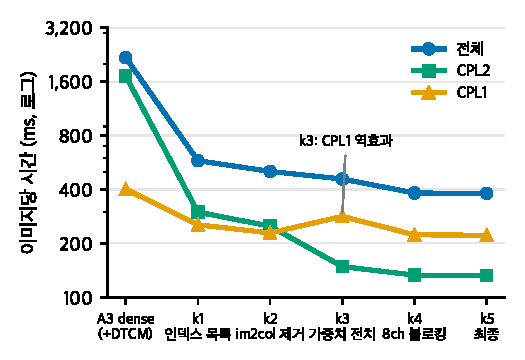
\includegraphics[width=0.95\linewidth]{figures/fig_kernel_iter.pdf}
\caption{희소 커널의 반복 개선 이력(로그 축). k3에서 CPL2는 크게
개선되나 CPL1이 퇴행하고, k4의 레지스터 블로킹이 양쪽을 회복한다.}
\label{fig:iter}
\end{figure}
